% ----------------------------------------------------------------
% To compile make sure you use pdflatex.  Once latex is installed
% on your system, you can invoke the following command from
% the command-line.
%
% >>> pdflatex hw-template.tex
%
% A successful compilation, will produce the file hw-template.pdf.
%
%
% The remaining part of the file is preamble stuff that you don't
% have to worry about.
%
%
% Head down to where it says "Start here"
% ----------------------------------------------------------------
 
\documentclass[11pt]{article}

\usepackage{fullpage} 
\usepackage{hyperref}
\usepackage{amsmath}
\usepackage{amssymb}
\usepackage{amsthm}
\usepackage{graphicx}
\usepackage{pgf}
\usepackage{tikz}
\usetikzlibrary{arrows,automata}


\newcommand{\question}[2] {\vspace{0.3in}\noindent{\subsection*{Question #1. #2} \vspace{0.15in}}}

\renewcommand{\part}[1] {{\vspace{0.15in}\noindent\textbf (#1)} \vspace{0.10in}}



%  ----------------------------------------------------------------
%                         Start here
% ----------------------------------------------------------------
 
\begin{document}

\title{Assignment \#2} %Replace X with the appropriate number
\author{\Large Gustavo Estrela de Matos\\ %Replace with your name
CSCE 433: Formal Languages and Automata} %If necessary, replace with your course number and title
\date{\today} 

\maketitle


\question{1}{Construct the NFA that accepts the language $\{w \vert w$ contains an odd number of 1's and exactly two 0's$\}$ with exatcly six states.}
First let's build a machine that accepts strings with odd number of 1's:

\begin{figure}[h]
\centering
\fbox{
    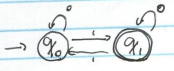
\includegraphics[scale=1.1]{ex1-1.png}
}
\end{figure}

Now we build a machine that accepts strings with exactly 2 zeros:

\begin{figure}[h]
\centering
\fbox{
    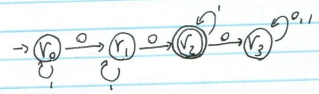
\includegraphics[scale=.9]{ex1-2.png}
}
\end{figure}

Notice that we used 6 states already. Then, since we don't need to keep track of strings that go to state $r_3$, we could simply remove this state, then all the strings with more than 2 zeros would halt on this machine.

Now we can create a new state that goes to both machines without consuming characters of the string:

\begin{figure}[h]
\centering
\fbox{
    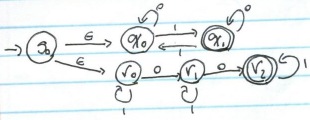
\includegraphics[scale=1]{ex1-3.png}
}
\end{figure}




\question{2}{Construct an NFA that accepts the set of binary strings that contain both substrings 010 and 101.}
A machine that accepts strings with both substrings $010$ and $101$ has either the substring $010$ or $101$ first, then we could build different machines for both cases:
\begin{itemize}

\item{$010$ and then $101$}

\begin{figure}[h]
\centering
\fbox{
    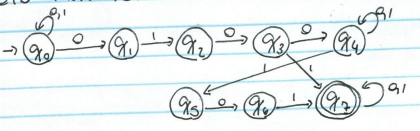
\includegraphics[scale=1]{ex2-3.png}
}
\end{figure}

Notice that the machine consider the case in which $010$ and $101$ overlaps.

\item{$101$ and then $010$}
\begin{figure}[h]
\centering
\fbox{
    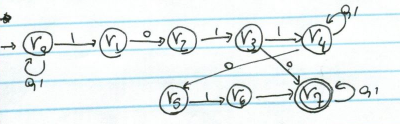
\includegraphics[scale=1]{ex2-4.png}
}
\end{figure}

\item{Which brings us to the final machine:}

\begin{figure}[h]
\centering
\fbox{
    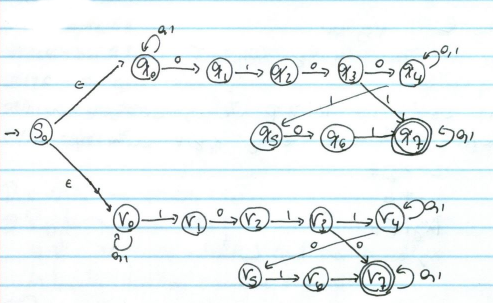
\includegraphics[scale=.9]{ex2-5.png}
}
\end{figure}

\end{itemize}





\question{3}{Convert the NFA below to a DFA}

\begin{figure}[h]
\centering
\fbox{
    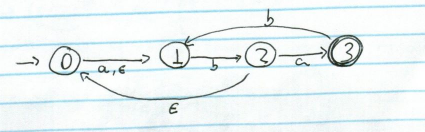
\includegraphics[scale=.8]{ex4.png}
}
\end{figure}

To solve this question we are going to use the same algorithm used to proove that $\epsilon$-NFAs are equivalent to DFAs. We are going to call this NFA $N = (Q, \Sigma, \delta, q, F)$ and build an equivalent DFA $M = (Q', \Sigma, \delta', q', F')$ such that $q' = C_{\epsilon}(0) = \{0, 1\}$; $\delta': \mathcal{P}(Q) \times \Sigma \rightarrow \mathcal{P}(Q)$ where $\delta'(R, a) = \bigcup \limits_{r \in R}^{} C_{\epsilon}(\delta(r, a))$ as it follows:

\begin{itemize}
\item{Start with the initial state}
\begin{figure}[h]
\centering
\fbox{
    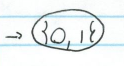
\includegraphics[scale=1]{ex3-1.png}
}
\end{figure}


\item{Calculate the transitions of $\{0, 1\}$}

$\delta'(\{0, 1\}, a) = C_{\epsilon}(1) \cup \emptyset = \{1\}$\\
$\delta'(\{0, 1\}, b) = \emptyset \cup C_{\epsilon}(2) = \{0, 1, 2\}$\\

\begin{figure}[h]
\centering
\fbox{
    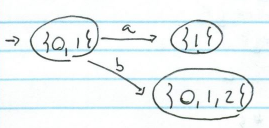
\includegraphics[scale=1]{ex3-2.png}
}
\end{figure}


\item{Calculate the transitions of \{1\} and \{0, 1, 2\}}

$\delta'(\{1\}, a) = \emptyset$\\
$\delta'(\{1\}, b) = C_{\epsilon}(2) = \{0, 1, 2\}$\\
$\delta'(\{0, 1, 2\}, a) = C_{\epsilon}(1) \cup \emptyset \cup C_{\epsilon}(3)= \{1, 3\}$\\
$\delta'(\{0, 1, 2\}, b) = \emptyset \cup C_{\epsilon}(2) \cup \emptyset = \{0, 1, 2\}$\\

\begin{figure}[ht!]
\centering
\fbox{
    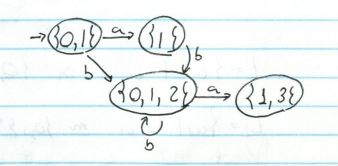
\includegraphics[scale=.8]{ex3-4.png}
}
\end{figure}

\newpage
\item{Calculate the transitions of \{1, 3\}}

$\delta'(\{1, 3\}, a) = \emptyset \cup \emptyset = \emptyset$\\
$\delta'(\{1, 3\}, b) = C_{\epsilon}(2) \cup C_{\epsilon}(1) = \{0, 1, 2\}$\\

\begin{figure}[h]
\centering
\fbox{
    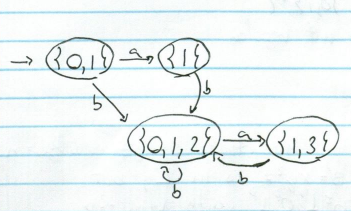
\includegraphics[scale=.8]{ex3-5.png}
}
\end{figure}
\end{itemize}




\question{4}{Prove that for every NFA with an arbitrary number of final states, there is an equivalent NFA with only one final state}

Let $N_1 = (Q_1, \Sigma, \delta_1, q_1, F_1)$ be an NFA with an arbitrary number of final states. We are going to build equivalent NFA $N_2 = (Q_2, \Sigma, \delta_2, q_2, F_2)$ with only one final state that is reachable from $N_1$ final states by $\epsilon$-transitions:

\begin{itemize}
\item{First we determine $F_2$, which should composed by just one state, then $F_2 = {q_f}$.}
\item{The inicial state stays the same $q_2 = q_1$.}
\item{The final state $q_f$ should be the only new state added to $N_1$, then $Q_2 = Q_1 \cup {q_f}$}
\item{Now we only need to determine $\delta_2: Q_2 \times \Sigma \rightarrow \mathcal{P}(Q_2)$ such that we keep the dynamics of $N_1$ and also add the $\epsilon$-transitions from the final states of $N_1$ to the new final state $f_2$}. Then we define:

\[
 \delta_2(q, a) =
  \begin{cases} 
      \hfill \delta_1(q, a) \cup \{q_f\}   \hfill & \text{ if $q \in F_1$ and $a = \epsilon$} \\
      \hfill \delta_1(q, a)                       \hfill & \text{ if $q \in Q_1$ and ($q \not \in F_1$ or $a \neq \epsilon$)}\\
      \hfill \emptyset       		     \hfill &  \text{otherwise}
  \end{cases}
\]
	
\end{itemize}




\question{5}{Give an inductive definition for the set S, of all strings in $\{0, 1\}^{\star}$ with an equal number of 0's and 1's}
\begin{itemize}
\item{\underline{Base case:}} $\epsilon \in S$
\item{\underline{Induction:}}  if $z \in S$, then $01z, 0z1, z01, 10z, 1z0$ and $z10$ are also in $S$
\end{itemize}

\question{6}{What is wrong with the following proof?}

\textbf{Proposition:} $6n = 0$ for all $n \in \mathbb{N}$

\begin{proof}
We will prove the above proposition by mathematical induction on $n \geq 0$.
\begin{itemize}
\item{\underline{\textit{Base case:}}} If $n = 0$, then $6n = 0$.

\item{\underline{\textit{Induction hypothesis:}}} Suppose that $6n = 0$ for $0 \leq n \leq k$.

\item{\underline{\textit{Induction step:}}} Let $n = k + 1 = a + b$, where $a$ and $b$ are natural numbers less than $k + 1$. \\
By induction hypothesis, $6a = 0$ and $6b = 0$. Therefore,
\begin{center}
$6n = 6(k + 1) = 6(a + b) = 6a + 6b = 0+ 0 = 0$
\end{center}
\end{itemize}
\end{proof}

The wrong statement in this proof is:
\begin{center}
\textit{
Let $n = k + 1 = a + b$, where $a$ and $b$ are natural numbers less than $k + 1$.
}
\end{center}
If we choose $n = 1$ we have that it is impossible to find $a$ and $b$ such that $a < 1$ and $b < 1$ and $a + b = 1$. Therefore everything that is stated on the existance of $a$ and $b$ can't be guaranteed to be true.


\end{document}

